% !TEX root = ../../ctfp-print.tex

\lettrine[lhang=0.17]{I}{t's about time} we had a little talk about sets.
Mathematicians have a love/hate relationship with set theory. It's the
assembly language of mathematics --- at least it used to be. Category
theory tries to step away from set theory, to some extent. For instance,
it's a known fact that the set of all sets doesn't exist, but the category
of all sets, $\Set$, does. So that's good. On the other hand, we assume that
morphisms between any two objects in a category form a set. We even
called it a hom-set. To be fair, there is a branch of category theory
where morphisms don't form sets. Instead they are objects in another
category. Those categories that use hom-objects rather than hom-sets,
are called \newterm{enriched} categories. In what follows, though, we'll
stick to categories with good old-fashioned hom-sets.

A set is the closest thing to a featureless blob you can get outside of
categorical objects. A set has elements, but you can't say much about
these elements. If you have a finite set, you can count the elements.
You can kind of count the elements of an infinite set using cardinal
numbers. The set of natural numbers, for instance, is smaller than the
set of real numbers, even though both are infinite. But, maybe
surprisingly, a set of rational numbers is the same size as the set of
natural numbers.

Other than that, all the information about sets can be encoded in
functions between them --- especially the invertible ones called
isomorphisms. For all intents and purposes isomorphic sets are
identical. Before I summon the wrath of foundational mathematicians, let
me explain that the distinction between equality and isomorphism is of
fundamental importance. In fact it is one of the main concerns of the
latest branch of mathematics, the Homotopy Type Theory (HoTT). I'm
mentioning HoTT because it's a pure mathematical theory that takes
inspiration from computation, and one of its main proponents, Vladimir
Voevodsky, had a major epiphany while studying the Coq theorem prover.
The interaction between mathematics and programming goes both ways.

The important lesson about sets is that it's okay to compare sets of
unlike elements. For instance, we can say that a given set of natural
transformations is isomorphic to some set of morphisms, because a set is
just a set. Isomorphism in this case just means that for every natural
transformation from one set there is a unique morphism from the other
set and vice versa. They can be paired against each other. You can't
compare apples with oranges, if they are objects from different
categories, but you can compare sets of apples against sets of oranges.
Often transforming a categorical problem into a set-theoretical problem
gives us the necessary insight or even lets us prove valuable theorems.

\section{The Hom Functor}

Every category comes equipped with a canonical family of mappings to
$\Set$. Those mappings are in fact functors, so they preserve the
structure of the category. Let's build one such mapping.

Let's fix one object $a$ in $\cat{C}$ and pick another object
$x$ also in $\cat{C}$. The hom-set $\cat{C}(a, x)$ is a set, an
object in $\Set$. When we vary $x$, keeping $a$
fixed, $\cat{C}(a, x)$ will also vary in $\Set$. Thus we have a
mapping from $x$ to $\Set$.

\begin{figure}[H]
\centering
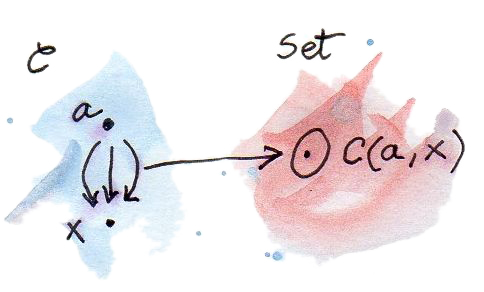
\includegraphics[width=0.45\textwidth]{images/hom-set.jpg}
\end{figure}

\noindent
If we want to stress the fact that we are considering the hom-set as a
mapping in its second argument, we use the notation $\cat{C}(a, -)$
with the dash serving as the placeholder for the argument.

This mapping of objects is easily extended to the mapping of morphisms.
Let's take a morphism $f$ in $\cat{C}$ between two arbitrary
objects $x$ and $y$. The object $x$ is mapped to
the set $\cat{C}(a, x)$, and the object $y$ is mapped to
$\cat{C}(a, y)$, under the mapping we have just defined. If this
mapping is to be a functor, $f$ must be mapped to a function
between the two sets: $\cat{C}(a, x) \to \cat{C}(a, y)$

Let's define this function point-wise, that is for each argument
separately. For the argument we should pick an arbitrary element of
$\cat{C}(a, x)$ --- let's call it $h$. Morphisms are
composable, if they match end to end. It so happens that the target of
$h$ matches the source of $f$, so their composition:
\[f \circ h \Colon a \to y\]
is a morphism going from $a$ to $y$. It is therefore a
member of $\cat{C}(a, y)$.

\begin{figure}[H]
\centering
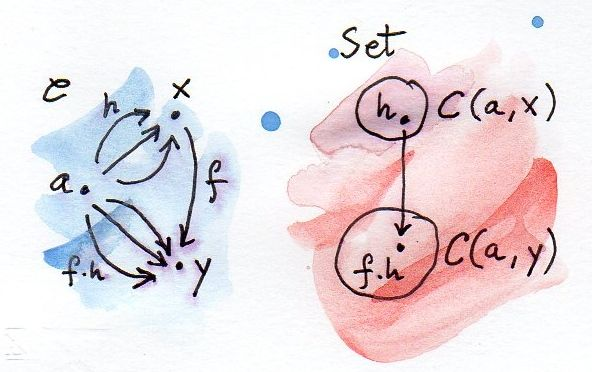
\includegraphics[width=0.45\textwidth]{images/hom-functor.jpg}
\end{figure}

\noindent
We have just found our function from $\cat{C}(a, x)$ to
$\cat{C}(a, y)$, which can serve as the image of $f$. If there
is no danger of confusion, we'll write this lifted function as: $\cat{C}(a, f)$
and its action on a morphism $h$ as:
\[\cat{C}(a, f) h = f \circ h\]
Since this construction works in any category, it must also work in the
category of Haskell types. In Haskell, the hom-functor is better known
as the \code{Reader} functor:

\src{snippet01}

\src{snippet02}
Now let's consider what happens if, instead of fixing the source of the
hom-set, we fix the target. In other words, we're asking the question if
the mapping $\cat{C}(-, a)$ is also a functor. It is, but instead of being covariant, it's
contravariant. That's because the same kind of matching of morphisms end
to end results in postcomposition by $f$; rather than
precomposition, as was the case with $\cat{C}(a, -)$.

We have already seen this contravariant functor in Haskell. We called it
\code{Op}:

\src{snippet03}

\src{snippet04}
Finally, if we let both objects vary, we get a profunctor
$\cat{C}(-, =)$, which is contravariant in the first argument and
covariant in the second (to underline the fact that the two arguments
may vary independently, we use a double dash as the second placeholder).
We have seen this profunctor before, when we talked about functoriality:

\src{snippet05}
The important lesson is that this observation holds in any category: the
mapping of objects to hom-sets is functorial. Since contravariance is
equivalent to a mapping from the opposite category, we can state this
fact succinctly as:
\[C(-, =) \Colon \cat{C}^{op} \times \cat{C} \to \Set\]

\section{Representable Functors}

We've seen that, for every choice of an object $a$ in $\cat{C}$,
we get a functor from $\cat{C}$ to $\Set$. This kind of
structure-preserving mapping to $\Set$ is often called a
\newterm{representation}. We are representing objects and morphisms of
$\cat{C}$ as sets and functions in $\Set$.

The functor $\cat{C}(a, -)$ itself is sometimes called representable.
More generally, any functor $F$ that is naturally isomorphic to
the hom-functor, for some choice of $a$, is called
\newterm{representable}. Such a functor must necessarily be
$\Set$-valued, since $\cat{C}(a, -)$ is.

I said before that we often think of isomorphic sets as identical. More
generally, we think of isomorphic \emph{objects} in a category as
identical. That's because objects have no structure other than their
relation to other objects (and themselves) through morphisms.

For instance, we've previously talked about the category of monoids,
$\cat{Mon}$, that was initially modeled with sets. But we were careful
to pick as morphisms only those functions that preserved the monoidal
structure of those sets. So if two objects in $\cat{Mon}$ are
isomorphic, meaning there is an invertible morphism between them, they
have exactly the same structure. If we peeked at the sets and functions
that they were based upon, we'd see that the unit element of one monoid
was mapped to the unit element of another, and that a product of two
elements was mapped to the product of their mappings.

The same reasoning can be applied to functors. Functors between two
categories form a category in which natural transformations play the
role of morphisms. So two functors are isomorphic, and can be thought of
as identical, if there is an invertible natural transformation between
them.

Let's analyze the definition of the representable functor from this
perspective. For $F$ to be representable we require that: There
be an object $a$ in $\cat{C}$; one natural transformation α from
$\cat{C}(a, -)$ to $F$; another natural transformation, β, in
the opposite direction; and that their composition be the identity
natural transformation.

Let's look at the component of α at some object $x$. It's a
function in $\Set$:
\[\alpha_x \Colon \cat{C}(a, x) \to F x\]
The naturality condition for this transformation tells us that, for any
morphism $f$ from $x$ to $y$, the following diagram
commutes:
\[F f \circ \alpha_x = \alpha_y \circ \cat{C}(a, f)\]
In Haskell, we would replace natural transformations with polymorphic
functions:

\src{snippet06}
with the optional \code{forall} quantifier. The naturality condition

\src{snippet07}
is automatically satisfied due to parametricity (it's one of those
theorems for free I mentioned earlier), with the understanding that
\code{fmap} on the left is defined by the functor $F$, whereas
the one on the right is defined by the reader functor. Since
\code{fmap} for reader is just function precomposition, we can be even
more explicit. Acting on $h$, an element of $\cat{C}(a, x)$,
the naturality condition simplifies to:

\src{snippet08}
The other transformation, \code{beta}, goes the opposite way:

\src{snippet09}
It must respect naturality conditions, and it must be the inverse of \code{alpha}:

\begin{snip}{text}
alpha . beta = id = beta . alpha
\end{snip}
We will see later that a natural transformation from $\cat{C}(a, -)$
to any $\Set$-valued functor always exists as long as $F a$ is 
non-empty (Yoneda's lemma) but it is not necessarily invertible.

Let me give you an example in Haskell with the list functor and
\code{Int} as \code{a}. Here's a natural transformation that does
the job:

\src{snippet10}
I have arbitrarily picked the number 12 and created a singleton list
with it. I can then \code{fmap} the function \code{h} over this list
and get a list of the type returned by \code{h}. (There are actually
as many such transformations as there are list of integers.)

The naturality condition is equivalent to the composability of
\code{map} (the list version of \code{fmap}):

\src{snippet11}
But if we tried to find the inverse transformation, we would have to go
from a list of arbitrary type \code{x} to a function returning
\code{x}:

\src{snippet12}
You might think of retrieving an \code{x} from the list, e.g., using
\code{head}, but that won't work for an empty list. Notice that there
is no choice for the type \code{a} (in place of \code{Int}) that
would work here. So the list functor is not representable.

Remember when we talked about Haskell (endo-) functors being a little
like containers? In the same vein we can think of representable functors
as containers for storing memoized results of function calls (the
members of hom-sets in Haskell are just functions). The representing
object, the type $a$ in $\cat{C}(a, -)$, is thought of as the
key type, with which we can access the tabulated values of a function.
The transformation we called \code{alpha} is called \code{tabulate}, and its
inverse, \code{beta}, is called \code{index}. Here's a (slightly simplified)
\code{Representable} class definition:

\src{snippet13}
Notice that the representing type, our $a$, which is called
\code{Rep f} here, is part of the definition of
\code{Representable}. The star just means that \code{Rep f} is a
type (as opposed to a type constructor, or other more exotic kinds).

Infinite lists, or streams, which cannot be empty, are representable.

\src{snippet14}
You can think of them as memoized values of a function taking an
\code{Integer} as an argument. (Strictly speaking, I should be using
non-negative natural numbers, but I didn't want to complicate the code.)

To \code{tabulate} such a function, you create an infinite stream of
values. Of course, this is only possible because Haskell is lazy. The
values are evaluated on demand. You access the memoized values using
\code{index}:

\src{snippet15}
It's interesting that you can implement a single memoization scheme to
cover a whole family of functions with arbitrary return types.

Representability for contravariant functors is similarly defined, except
that we keep the second argument of $\cat{C}(-, a)$ fixed. Or,
equivalently, we may consider functors from $\cat{C}^{op}$
to $\Set$, because $\cat{C}^{op}(a, -)$ is the same as
$\cat{C}(-, a)$.

There is an interesting twist to representability. Remember that
hom-sets can internally be treated as exponential objects, in Cartesian
closed categories. The hom-set $\cat{C}(a, x)$ is equivalent to
$x^a$, and for a representable functor $F$ we can write: $-^a = F$.

Let's take the logarithm of both sides, just for kicks: $a = \mathbf{log}F$

Of course, this is a purely formal transformation, but if you know some
of the properties of logarithms, it is quite helpful. In particular, it
turns out that functors that are based on product types can be
represented with sum types, and that sum-type functors are not in
general representable (example: the list functor).

Finally, notice that a representable functor gives us two different
implementations of the same thing --- one a function, one a data
structure. They have exactly the same content --- the same values are
retrieved using the same keys. That's the sense of ``sameness'' I was
talking about. Two naturally isomorphic functors are identical as far as
their contents are involved. On the other hand, the two representations
are often implemented differently and may have different performance
characteristics. Memoization is used as a performance enhancement and
may lead to substantially reduced run times. Being able to generate
different representations of the same underlying computation is very
valuable in practice. So, surprisingly, even though it's not concerned
with performance at all, category theory provides ample opportunities to
explore alternative implementations that have practical value.

\section{Challenges}

\begin{enumerate}
\tightlist
\item
  Show that the hom-functors map identity morphisms in \emph{C} to
  corresponding identity functions in $\Set$.
\item
  Show that \code{Maybe} is not representable.
\item
  Is the \code{Reader} functor representable?
\item
  Using \code{Stream} representation, memoize a function that squares
  its argument.
\item
  Show that \code{tabulate} and \code{index} for \code{Stream} are
  indeed the inverse of each other. (Hint: use induction.)
\item
  The functor:

\begin{snip}{haskell}
Pair a = Pair a a
\end{snip}
  is representable. Can you guess the type that represents it? Implement
  \code{tabulate} and \code{index}.
\end{enumerate}

\section{Bibliography}

\begin{enumerate}
\tightlist
\item
  The Catsters video about
  \urlref{https://www.youtube.com/watch?v=4QgjKUzyrhM}{representable
  functors}.
\end{enumerate}
